%% Follow comments to support use.

%%%%%%%%%%%%%%%%%%%%%%%%%%%%%%%%%%%%%%%%%%%%%%%%%%%%%%%%%
%% STEP 1: Choose options for MSc / BSc / seminar layout and your bibliographic style
%%%%%%%%%%%%%%%%%%%%%%%%%%%%%%%%%%%%%%%%%%%%%%%%%%%%%%%%%

%%  Language: 
%%      finnish, swedish, or english
%%  Pagination (use twoside by default)  
%%      oneside or twoside,
%%  Study programme / kind of report
%%      csm  = Master's thesis in Computer Science Master's Programme;
%%      tkt = Bachelor's thesis in Computer Science Bachelor's Programme;
%%      seminar = seminar report
%%  For Master's thesis choose your line or track:
%%      (30 cr thesis, 2020 onwards, Master's Programme in Computer Science = csm)
%%      software-track-2020 = Software study track
%%      algorithms-track-2020 = Algorithms study track
%%      networking-track-2020 = Networking study track

\documentclass[english,twoside,censored,csm,software-track-2020]{HYthesisML} 


% If wanted, open new chapters only at right page.
% By default, "openany".
%\PassOptionsToClass{openright,twoside,a4paper}{report}
\PassOptionsToClass{openany,twoside,a4paper}{report}

\usepackage{csquotes}
%%%%%%%%%%%%%%%%%%%%%%%%%%%%%%%%%%%%%%%%%%%%%%%%%%%%%%%%%
%% REFERENCES
%% Some notes on bibliography usage and options:
%% natbib -> you can use, e.g., \citep{} or \parencite{} for (Einstein, 1905); with APA \cite -> Einstein, 1905 without ()
%% maxcitenames=2 -> only 2 author names in text citations, if more -> et al. is used
%% maxbibnames=99 as no great need to suppress the biliography list in a thesis
%% for more information see biblatex package documentation, e.g., from https://ctan.org/pkg/biblatex 

%% Reference style: select one 
%% for APA = Harvard style = authoryear -> (Einstein, 1905) use:
\usepackage[style=authoryear,bibstyle=authoryear,backend=biber,natbib=true,maxnames=99,maxcitenames=2,uniquelist=minyear,giveninits=true,uniquename=mininit]{biblatex}
%% for numeric = Vancouver style -> [1] use:
%\usepackage[style=numeric,bibstyle=numeric,backend=biber,natbib=true,maxbibnames=99,giveninits=true,uniquename=init]{biblatex}
%% for alpahbetic -> [Ein05] use:
%\usepackage[style=alphabetic,bibstyle=alphabetic,backend=biber,natbib=true,maxbibnames=99,giveninits=true,uniquename=init]{biblatex}
%

\addbibresource{bibliography.bib}
% in case you want the final delimiter between authors & -> (Einstein & Zweistein, 1905) 
% \renewcommand{\finalnamedelim}{ \& }
% List the authors in the Bibilipgraphy as Lastname F, Familyname G,
\DeclareNameAlias{sortname}{family-given}
% remove the punctuation between author names in Bibliography 
%\renewcommand{\revsdnamepunct}{ }


%% Block of definitions for fonts and packages for picture management.
%% In some systems, the figure packages may not be happy together.
%% Choose the ones you need.

%\usepackage[utf8]{inputenc} % For UTF8 support, in some systems. Use UTF8 when saving your file.

\usepackage{lmodern}         % Font package, again in some systems.
\usepackage{textcomp}        % Package for special symbols
\usepackage[pdftex]{color, graphicx} % For pdf output and jpg/png graphics
\usepackage{epsfig}
\usepackage{subfigure}
\usepackage[pdftex, plainpages=false]{hyperref} % For hyperlinks and pdf metadata
\usepackage{fancyhdr}        % For nicer page headers
\usepackage{tikz}            % For making vector graphics (hard to learn but powerful)
%\usepackage{wrapfig}        % For nice text-wrapping figures (use at own discretion)
\usepackage{amsmath, amssymb} % For better math

\singlespacing               %line spacing options; normally use single

\fussy
%\sloppy                      % sloppy and fussy commands can be used to avoid overlong text lines
% if you want to see which lines are too long or have too little stuff, comment out the following lines
% \overfullrule=1mm
% to see more info in the detailed log about under/overfull boxes...
% \showboxbreadth=50 
% \showboxdepth=50



%%%%%%%%%%%%%%%%%%%%%%%%%%%%%%%%%%%%%%%%%%%%%%%%%%%%%%%%%
%% STEP 2:
%%%%%%%%%%%%%%%%%%%%%%%%%%%%%%%%%%%%%%%%%%%%%%%%%%%%%%%%%
%% Set up personal information for the title page and the abstract form.
%% Replace parameters with your information.
\title{Case study: Performance of JavaScript on server side}

\author{Nicolas J, Valentine}
\date{\today}

% Set supervisors, use the titles according to the thesis language
% in English Prof. or Dr., or in Finnish toht. or tri or FT, TkT, Ph.D. or in Swedish... 
\supervisors{A.P.~Tuovinen}

\keywords{software}
\additionalinformation{\translate{\track}}

%% For seminar reports:
%%\additionalinformation{Name of the seminar}

%% Provide classification terms, to appear on the abstract page.
%% Replace the classification terms below with the ones that match your work.
%% ACM Digital library provides a taxonomy and a tool for classification
%% in computer science. Use 1-3 paths, and use right arrows between the
%% about three levels in the path; each path requires a new line.

\classification{\protect{\ \\
\  General and reference $\rightarrow$ Document types  $\rightarrow$ Surveys and overviews\  \\
\  Applied computing  $\rightarrow$ Document management and text processing  $\rightarrow$ Document management $\rightarrow$ Text editing
}}

%% If you want to quote someone special. You can comment this line out and there will be nothing on the document.
%\quoting{Bachelor's degrees make pretty good placemats if you get them laminated.}{Jeph Jacques}


%% OPTIONAL STEP: Set up properties and metadata for the pdf file that pdfLaTeX makes.
%% Your name, work title, and keywords are recommended.
\hypersetup{
    unicode=true,           % to show non-Latin characters in Acrobat’s bookmarks
    pdftoolbar=true,        % show Acrobat’s toolbar?
    pdfmenubar=true,        % show Acrobat’s menu?
    pdffitwindow=false,     % window fit to page when opened
    pdfstartview={FitH},    % fits the width of the page to the window
    pdftitle={},            % title
    pdfauthor={Nicolas Valentine},           % author
    pdfsubject={},          % subject of the document
    pdfcreator={},          % creator of the document
    pdfproducer={pdfLaTeX}, % producer of the document
    pdfkeywords={something} {something else}, % list of keywords for
    pdfnewwindow=true,      % links in new window
    colorlinks=true,        % false: boxed links; true: colored links
    linkcolor=black,        % color of internal links
    citecolor=black,        % color of links to bibliography
    filecolor=magenta,      % color of file links
    urlcolor=cyan           % color of external links
}

%%-----------------------------------------------------------------------------------

\begin{document}

% Generate title page.
\maketitle

%%%%%%%%%%%%%%%%%%%%%%%%%%%%%%%%%%%%%%%%%%%%%%%%%%%%%%%%%
%% STEP 3:
%%%%%%%%%%%%%%%%%%%%%%%%%%%%%%%%%%%%%%%%%%%%%%%%%%%%%%%%%
%% Write your abstract in the separate file, to be positioned here.
%% You can make several abstract pages (if you want it in different languages),
%% in which case you should also define the language of the abstract,
%% as below.

% \begin{abstract}{finnish}

% Tämä dokumentti on tarkoitettu Helsingin yliopiston tietojenkäsittelytieteen osaston opin\-näyt\-teiden ja harjoitustöiden ulkoasun ohjeeksi ja mallipohjaksi. Ohje soveltuu kanditutkielmiin, ohjelmistotuotantoprojekteihin, seminaareihin ja maisterintutkielmiin. Tämän ohjeen lisäksi on seurattava niitä ohjeita, jotka opastavat valitsemaan kuhunkin osioon tieteellisesti kiinnostavaa, syvällisesti pohdittua sisältöä.


% Työn aihe luokitellaan  
% ACM Computing Classification System (CCS) mukaisesti, 
% ks.\ \url{https://dl.acm.org/ccs}. 
% Käytä muutamaa termipolkua (1--3), jotka alkavat juuritermistä ja joissa polun tarkentuvat luokat erotetaan toisistaan oikealle osoittavalla nuolella.

% \end{abstract}

\begin{otherlanguage}{english}
\begin{abstract}
A case study that studied the performance impact of a node.js component when it was refactored from monolith environment into independent service.
The performance study studied the response time of the blocking part of JavaScript code in the component.
The non blocking part of the code and the added network overhead from the refactoring were excluded from the performance review.

Literature review didn't show any related research that studied the performance impact of a node.js component when it was refactored from monolith into microservices.
Many found studies were found that studied the response time and throughput of REST API build with node.js with comparisons to other programming languages.
A study were found that related to refactoring an application from monolith into microservices.
None of the found studies were directly related to the studied case.

It was noted that the response time of the component improved by $46.5\%$ when it was refactored from monolith into microservice.
It is possible that when a node.js monolith application grows it starts to affect the throughput of the event loop affecting performance critical components.
For the case component it was beneficial to refactor it into independent service in order to gain the $92.6$ms in the mean response time.


\end{abstract}
\end{otherlanguage}


% Place ToC
%\newpage
\mytableofcontents

\mainmatter

%%%%%%%%%%%%%%%%%%%%%%%%%%%%%%%%%%%%%%%%%%%%%%%%%%%%%%%%%
%% STEP 4: Write the thesis.
%%%%%%%%%%%%%%%%%%%%%%%%%%%%%%%%%%%%%%%%%%%%%%%%%%%%%%%%%
%% Your actual text starts here. You shouldn't mess with the code above the line except
%% to change the parameters. Removing the abstract and ToC commands will mess up stuff.
%%
%% Command \include{file} includes the file of name file.tex.
%% A new page will be created at every \include command, 
%% which makes it appropriate to use it for large entities such as book chapters. Cannot be nested.
%% It is useful for a big project, as changing one of the include targets 
%% won't force the regeneration of the outputs of all the rest.
%% Alternatively, \input is a more lower level macro 
%% which simply inputs the content of the given file like it was copy&pasted there manually.

\chapter{Introduction\label{intro}}

Introduction to the topic.

A case study to measure response time of JavaScript application in different environments. 

\subsubsection{Motivation}

\subsubsection{Intentions}

\subsubsection{Cause relation}


\section{Related work}
Related studies, JavaScript benchmarks etc...
\chapter{Background\label{background}}
This chapter gives background information on the related technologies and architectural patterns.


\section{JavaScript}
- How it works?

- How it differs from other languages?


\subsection{V8 - JavaScript engine}
- how it works

- how it handles different situations

-- performance

-- where it is used





\subsection{Node.js}

\begin{center}
\begin{tabular}{|c c|} 
 \hline
 Node.js version & V8 version \\ [0.5ex] 
 \hline
 14.18.3 & 8.4.371.23-node.85  \\ 
 \hline
  14.19.1 & 8.4.371.23-node.85  \\ 
 \hline
\end{tabular}
\end{center}

- what is

- how it works

- performance

-- performance of different versions











\section{Architecture}

\subsection{Monolith}
What is a monolith?

\subsection{Microservices}
What is microservice?

\chapter{The Case\label{case}}

\section{Architecture}
The studied application was build following monolith architecture with three tier pattern containing frontend, backend and database.
The backend was written using node.js version v14.19.1 that uses V8 engine version \textit{8.4.371.23-node.85}.
The backend contains multiple independent components each with its own purpose.
One of the components were refactored out of the monolith application into the independent service.

The independent service contained an application interface to allow communication to the component and the component itself.
The independent service was build using node.js with version v14.18.3 that uses V8 engine version \textit{8.4.371.23-node.85}.
The architecture before and after refactoring can be seen in figures \ref{figure:architecture:monolith} and \ref{figure:architecture:independent_service}.

\begin{figure}
    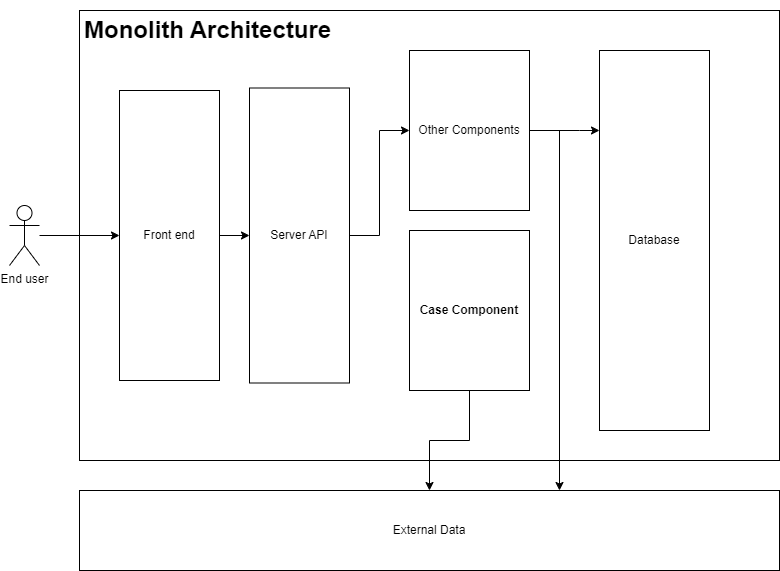
\includegraphics[width=\textwidth]{images/monolith_architecture.png}
    \caption{Architectural overview of the application before refactoring.}
    \label{figure:architecture:monolith}
\end{figure}
\begin{figure}
    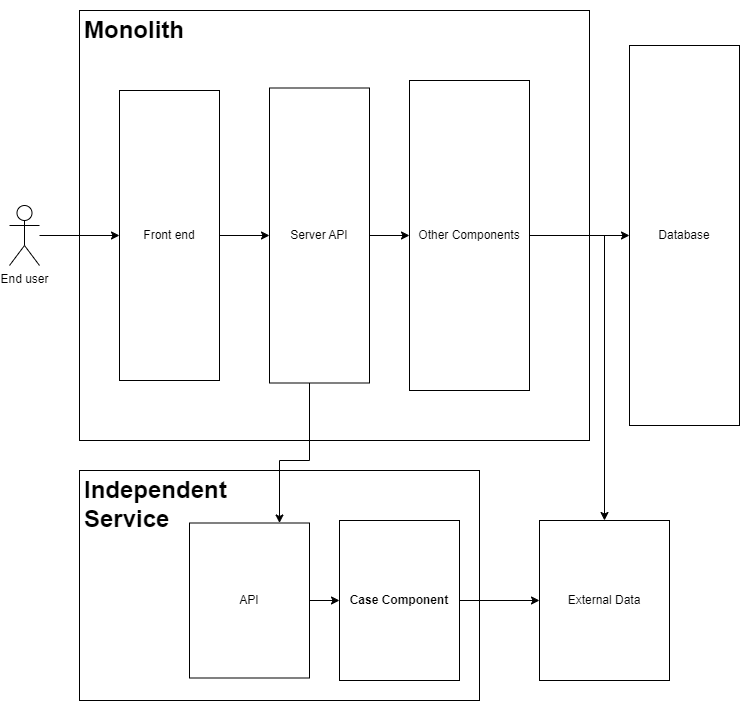
\includegraphics[width=\textwidth]{images/independent_service_arcitecture.png}
    \caption{Architectural overview of the application after refactoring the component into independent service.}
    \label{figure:architecture:independent_service}
\end{figure}

Both environments, the monolith and the independent service, were running in linux server provided by amazon web services.
The hardware specifications were different in both environment.
The monolith environment had 64GB RAM with 8 vCPU of computing power while the independent service had 4GB RAM with 1 vCPU of computing power available.
The use of production environment didn't allow to utilize same resources for both environments.

\begin{table}[h!]
    \begin{tabular}{|c|c|c|c|c|} 
        \hline
        Environment
        & RAM (GB)
        & Core (vCPU)
        & Node.js version
        & V8 version
        \\ 
        \hline\hline
        Monolith
        & 64GB
        & 8
        & v14.19.1
        & 8.4.371.23-node.85
        \\
        Independent service
        & 8GB
        & 1
        & 14.18.3
        & 8.4.371.23-node.85
        \\
        \hline
    \end{tabular}    
    \caption{Hardware specification.}
    \label{represented:harware:specs}
\end{table}

\section{Overview of the Component}
The component was written using javascript with node.js runtime environment.
The component runs in cycles where one cycle contains two to four tasks.
After a cycle is finished the component decides if it start new cycle.
The cycles keeps running until user interrupts the cycles or and error stops the process.

The component is divided into four modules each handling one of the four task.
Each task is represented by its own module and each module is run sequentially one after the other
all of the modules response time is critical to the system.
\begin{itemize}
    \item
    \textbf{Module A} is the first module in the cycle.
    It is always called when the cycles are running.
    
    \item
    \textbf{Module B} is the second module in the cycle.
    It runs after \textbf{module A}.
    
    \item
    \textbf{Module C} is the third module in the cycle.
    It runs after \textbf{module B} only when the response from \textbf{module A} requires it to run.
    Otherwise rest of the modules in the cycle are skipped and the cycle restarts from \textbf{module A}.

    \item
    \textbf{Module D} is the last module in the cycle.
    After it is finished the cycle is restarted from \textbf{module A}.
\end{itemize}

The components is dependent on the user input that decides if the component is running or not.
Modules A, C and D are dependent on external data.
Module D is dependent on module C and module C is dependent on module A.
The dependencies of the modules can be seen in figure \ref{figure:module:relation}.
The flowchart of the modules are shown in figure \ref{figure:module:flow}.

\begin{figure}
    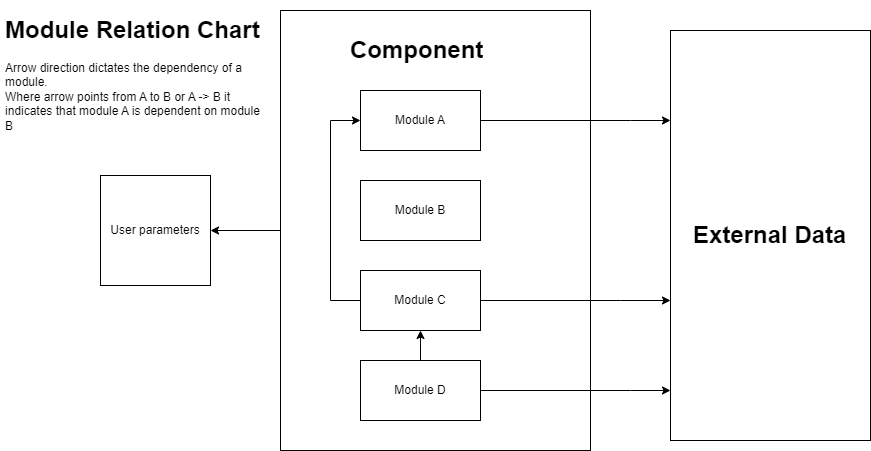
\includegraphics[width=\textwidth]{images/modules_relation_uml.png}
    \caption{Components modules and their dependencies.}
    \label{figure:module:relation}
\end{figure}


\begin{figure}
    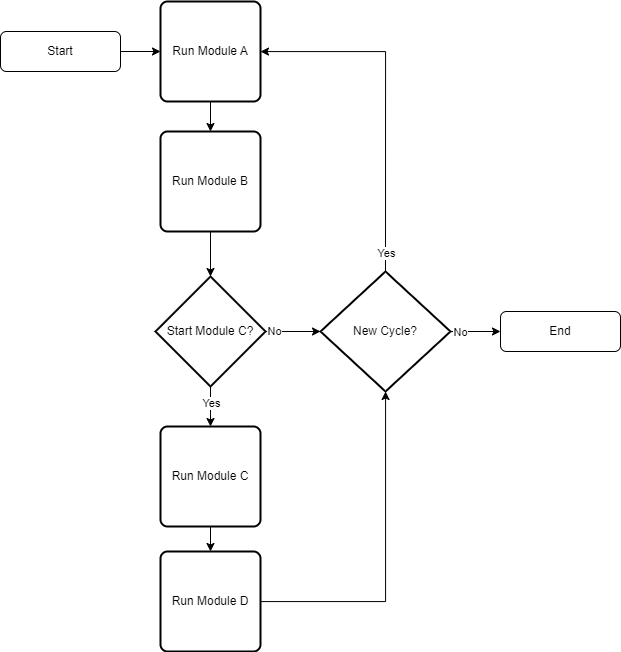
\includegraphics[width=\textwidth]{images/module_flow_chart.png}
    \caption{Modules flowchart. Modules are run inside the studied component.}
    \label{figure:module:flow}
\end{figure}

When any of the modules fails to perform its task an error is raised and the cycle is interrupted.
Error at any point of the cycles requires manual restart from the user.
When modules are running without errors the modules A and B are always performed. 
The modules C and D are run only when the data from \textbf{module A} requires them to run.
Each module waits for the response of external calls before continuing their process.
A full cycle requires succesful run from all four modules.

This research studies performance of a server side JavaScript software component.
Performance is defined as the time the component takes to processing its blocking events.
All non blocking calls from the component are timed and excluded from the performance review in order to capture the response time of all blocking events in the component.
The component performance is measured when it is a part of a monolith application and when it is refactored into its own service.
The component is not modified between environments.
The components performance is critical tot he system.

\chapter{Methods\label{methods}}

\section{Research questions}

To find out if there is any significant difference in the server side JavaScript components response time three research questions are defined to answer these questions.

\begin{itemize}
    \item RQ1\label{RQ1}: What is the response time of a server side monolith JavaScript application?
    \item RQ2\label{RQ2}: What is the response time of a server side independent JavaScript service?
    \item RQ3\label{RQ3}: What is the relation of the response time in different environments?
\end{itemize}

The first research question (RQ1) aims to provide data related to the response time of JavaScript component. The component is running as part of the monolith application.

The second research question (RQ2) aims to provide data related to the response time of JavaScript component. The component is running as an independent service.

The third research question (RQ3) provides statistical analysis based on the data provided by the first (RQ1) and second (RQ2) research questions.

\section{Literature}
To find out about existing literature related to the case a two phase hybrid search was performed.
First phase contained a modified systematic literature review with predefined keywords.
The seconds phase used snowballing method with one iteration on the literature found on first phase.
One iteration consisted one back step and one forward step for each final results from phase one.

\subsection{Literature review}
The first search phase is a literature review to find out relevant literature to the case.

\subsubsection{Review protocol}
To find out about related research a five step literature review was implemented.

\begin{enumerate}
    \item Define the review protocol.
    \item Search literature based on the protocol.
    \item Filter results by title and meta-data.
    \item Review findings abstracts by criteria.
    \item Analyze relevant results.
\end{enumerate}

The first step defines the protocol used in the search.

The second step search for the related research based on the protocol.

The third step performs the first analysis of the results to find out relevant research.

The fourth step reviews filtered articles and gives the a quality score.

The fifth steps performs the analysis of the results from the fourth step.



 search the following key words
For each search engine we performed search using the following search string: 

Results analysis.
Point system for inclusion/exclusion.


\subsubsection{The search}
The search was performed on the following search engines: 
\begin{itemize}
    \item 1. search engine
    \item ...
\end{itemize}.

The search was performed on the title, abstract and meta-data for the following key words: \textbf{KEY\_WORDS}.
For each search engine we used \textbf{SEARCH\_STRING} to find out related research.
Only research from years \textbf{YEARS} was included.

The search returned \textbf{HITS} hits.
\textbf{TABLE\_WITH\_RESULTS\_PER\_ENGINE}


\subsubsection{Initial filtering}
The relevance of the each results was analyzed based on the title and meta-data related to the keywords. Each result was given score based on the point system.

\subsubsection{Quality Review}
Then the quality of found articles from the initial filtering was performed.
Each article was review based on the review criteria and abstract.
Each criteria was scored based on the point system.

For reviewing the relevance of the articles each articles abstract was reviewed.

\begin{flushleft}
\begin{tabular}{|c c|} 
 \hline
 Criteria & Description \\ [0.5ex] 
 \hline
  Cr.1 & JavaScript performance review  \\ 
  \hline
  Cr.2 & Node.js performance review  \\ 
  \hline
  Cr.3 & Architectural performance review  \\ 
  \hline
  Cr.4 & Response time performance review  \\ 
  \hline
  Cr.5 & Server side performance review  \\ 
  \hline
\end{tabular}
\end{flushleft}


\begin{flushleft}
\begin{tabular}{|c c|} 
 \hline
 Points & Description \\ [0.5ex] 
 \hline
  0 & No relevance to the criteria  \\ 
 \hline
  0.5 & Some relevance to the criteria \\ 
 \hline
 1 & Relevant to the criteria \\ 
 \hline
\end{tabular}
\end{flushleft}

\textbf{A table of results and total points}

\subsubsection{Final result}
For the final results only articles with the relevance point at or above \textbf{relevance point threshold} was included.

The final results with the quality score can be found in the \textbf{TABLE}.

Add tables of results grouped by relevant data, category, relevance score, quality score.

\subsection{Snowballing - Phase two}
The snowballing method was performed on the final results from phase one.
The method included 
\begin{enumerate}
    \item All references from phase one results.
    \item Research that used previous steps results as reference.
    \item The initial filtering was performed on the all found result.
    \item Each result was review for their quality.
    \item Final result was analyzed. 
\end{enumerate}

The result can be found in the \textbf{reference table}.

\section{Data}
% What data was collected?
To measure the response time of the case a series of data points were collected from the component.
The data points were collected from two environments.
First environment was integrated as a part of the monolith application.
Second environment contained the component and the restful service for communication.

The measured data contains run-time information about the module.
A single data point contains five values.
\begin{enumerate}
    \item Cycle id
    \item Timestamp id
    \item System time (in nanoseconds)
    \item System free memory
    \item System total memory
    \item Used process CPU percentage
\end{enumerate}

The cycle id is unique for each full component cycle.
The memory and CPU usages were collected to ensure that the system had enough resources to operate.
Data points were collected at the beginning of the application cycle, at the end of the cycle and before and after each third party or internal function call.

For each environment the data was saved at run-time and persisted at the end of each cycle.
Sometimes the cycle can be interrupted by an error.
Only data points from full cycles were included.

\textbf{Table about how many total data points per environment and how many full cycles}

\textbf{Table containing mean, standard deviation, sample size and standard error for each module, environment and external calls for each environment}




% What data was included and what excluded? And reasons

% What data sources are used and why?


% How data from the modules was collected

% How data was analysed

% How the data can answer the research questions

% How case size (data points) was defined



\chapter{Results\label{results}}
The performed literature review results and the collected data analysis is described in this chapter.

\section{Literature Review}
Literature review was performed to find related literature to \textbf{RQ1}.
Review used four search engines that provided 147 initial results when using defined search string.
From the 147 initial search results 93 were unique.
\begin{table}[ht!]
    \begin{tabular}{|c c|} 
        \hline
        Search Engine
        & Search Hits
        \\ 
        \hline\hline
        Helka (University of Helsinki library)
        & 46
        \\ 
        
        IEEE Xplore
        & 26
        \\ 
        
        Google Scholar
        & 7
        \\ 
        
        Scopus
        & 68
        \\ 
        \hline
        Total
        & 147
        \\ 
        \hline
    \end{tabular}    
    \caption{Initial search results of related literature}
    \label{table:literature:initialSearchResults}
\end{table}
Search results title and abstract was reviewed against inclusion criteria.
Highest score received was 8 out of 14 for three unique results and lowest score 0 out of 14 for 24 unique results.
Three results didn't have an abstract to review so they were excluded from the review at this point.
Table \ref{table:literature:inclusionResults} shows inclusion score among initial search results.
\begin{table}[ht!]
    \begin{tabular}{|c c c c|} 
        \hline
        Inclusion Score
        & Count (n)
        & Unique Count (n)
        & Included Literature Id
        \\ 
        \hline\hline
        Score 8/14
        & 7
        & 3
        & 1, 2, 3
        \\ 
        
        Score 7/14
        & 4
        & 2
        & All excluded
        \\ 
        
        Score 6/14
        & 4
        & 4
        & 4
        \\ 
        
        Score 5/14
        & 16
        & 8
        & 5, 6, 7, 8
        \\ 
        
        Score 4/14
        & 17
        & 11
        & 9, 10, 11, 12
        \\ 
        
        Score 3/14
        & 23
        & 14
        & All excluded
        \\ 
        
        Score 2/14
        & 36
        & 20
        & All excluded
        \\ 
        
        Score 1/14
        & 9
        & 4
        & All excluded
        \\ 
        
        Score 0/14
        & 28
        & 24
        & All excluded
        \\ 
        
        Not available
        & 3
        & 3
        & Not included
        \\ 
        \hline
        Total
        & 147
        & 93
        & 12
        \\ 
        \hline
    \end{tabular}    
    \caption{Literature inclusion scores}
    \label{table:literature:inclusionResults}
\end{table}
After excluding results with inclusion score less than 3.5 a total of 28 unique results were review.
Out of the 28 included results 16 were excluded based on exclusion criteria leaving a total of 12 results relevant to \textbf{RQ1} as shown in table \ref{table:literature:results}.
As shown in table \ref{table:literature:resulstByCategory} most of the found literature, $50\%$, compares node.js web server with other programming languages like .net, python and PHP.
One results studied performance impact when monolith application was migrated to microservice.
Other study studied the performance impact of JavaScript API with different JavaScript engines.

\begin{table}[ht!]
    \begin{tabular}{|c c |} 
        \hline
        Literature Id
        & Citation
        \\ 
        \hline\hline
        1
        & \cite{Dafni}
        \\ 
        
        2
        & \cite{Tilkov}
        \\ 
        
        3
        & \cite{Chitra}
        \\ 
        
        4
        & \cite{Shkodra}
        \\ 
        
        5
        & \cite{Chaniotis}
        \\ 
        
        6
        & \cite{NkenyereyeLionel2016PEoN}
        \\ 
        
        7
        & \cite{faustino}
        \\ 
        
        8
        & \cite{Challapalli}
        \\ 
        
        9
        & \cite{Kyriakou}
        \\ 
        
        10
        & \cite{Kyriakou}
        \\ 
        
        11
        & \cite{Lei}
        \\ 
        
        12
        & \cite{SelakovicPerformanceIssues}
        \\ 
        \hline
    \end{tabular}    
    \caption{Literature review results.}
    \label{table:literature:results}
\end{table}


\begin{table}[ht!]
    \begin{tabular}{|c c|} 
        \hline
        Category
        & Literature Id
        \\ 
        \hline\hline
        Node.js I/O performance
        & 1, 10, 11
        \\ 
    
        Description of Node.js as network program
        & 2
        \\ 
    
        Node.js benchmarks
        & 5, 6, 10
        \\ 
    
        Node.js IoT server
        & 6
        \\ 
    
        Migration from monolith to microservice
        & 7
        \\ 
    
        Achieving efficient power usage by scaling CPU frequency
        & 10
        \\ 
    
        Inefficient usage of JavaScript internal APIs effects to performance
        & 12
        \\ 
    
        Comparison of node.js web server with other programming language
        & 3, 4, 5, 8, 9, 11
        \\ 
    
        Comparison against PHP/Apache
        & 5
        \\ 
    
        Comparison against PHP
        & 11
        \\ 
    
        Comparison against Nginx
        & 5
        \\
    
        Comparison against .NET
        & 3, 4
        \\
    
        Comparison against python
        & 8, 11
        \\
    
        Comparison against rust
        & 9
        \\
    
        Comparison against web assembly
        & 9
        \\
        \hline
    \end{tabular}    
    \caption{Literature results by category.}
    \label{table:literature:resulstByCategory}
\end{table}

\section{Sample Data}
Performance samples were collected from the component in both environments sequentially over two month period.
In order to capture the component performance only full cycles were included in the analysis.
Partial cycles and cycles with errors were excluded from the samples since the performance in these cases was irrelevant to the system.
Hardware samples are shown in tables \ref{table:hardware results:monolith:1} and \ref{table:hardware results:independent service:1}.
The response time samples are shown in tables \ref{table:response time results:1}, \ref{table:response time results:2} and \ref{table:response time results:3}.

\subsubsection{Hardware Samples}
Hardware samples were collected along each cycle to make sure that the components response time was not limited by the used hardware.
Only samples from full cycles without errors were included.
The results for monolith are shown in table \ref{table:hardware results:monolith:1} and for independent service in table \ref{table:hardware results:independent service:1}.
In the monolith environment $206965$ hardware samples was collected from $1649$ full cycles.
From the independent service a total of $26902$ hardware samples was collected from $205$ full cycles.
The hardware samples were collected along response time timestamps.
Hardware samples only reflects the systems CPU utilization and memory usage at the point of the timestamp collection and not the status during any meaningful process in the component.

\begin{table}[ht!]
    \begin{tabular}{|c c c c|} 
        \hline
        Monolith
        & CPU (\%)
        & Free Memory (Gigabytes)
        & Total Memory (Gigabytes) \\ [0.5ex] 
        
        \hline\hline
        Mean
        & 25.0
        & 7.588166...
        & 64.265863... \\ 
        
        Median
        & 22.0
        & 3.699269...
        & 64.265863... \\ 

        Minimum
        & 6.0
        & 0.391187...
        & 64.265863... \\ 
        
        Maximum
        & 36.0
        & 55.782023...
        & 64.265863... \\
        \hline
    \end{tabular}
    \caption{Hardware Utilization - Monolith $n=206 965$}
    \label{table:hardware results:monolith:1}
\end{table}

Collected hardware samples shows the systems CPU utilization percentage.
The CPU utilization percentage was calculated as
\[
\textit{Utilization percentage} = 100 \cdot \frac{\textit{Available CPU}}{\textit{Total CPU}}
.\]
Where available CPU is the number of milliseconds the system has spend in the user mode.
The total CPU is the sum of milliseconds the system has spend on user, system and idle modes. The CPU utilization is shown in tables \ref{table:hardware results:monolith:1} and \ref{table:hardware results:independent service:1}.

Collected samples shows that the CPU utilization percentage didn't have any noted effect on the performance since the maximum CPU utilization was at $36.0\%$ in the monolith environment and $1.0\%$ in the independent service.
Leaving most of the CPU available to the application process.
The mean CPU utilization in the monolith is 24 percentage points higher compared to the mean CPU utilization in the independent service.

Collected hardware samples contained information about the free memory and the total available memory for the system.
In table \ref{table:hardware results:monolith:1} the memory data is shown for the monolith application and in table \ref{table:hardware results:independent service:1} for the independent service.
The minimum available memory for the system in monolith was around $0.609...\%$ and in independent service around $61.233...\%$.
Minimum available memory was calculated with the following formula:
\[
\textit{Minimum available memory} = 100 \cdot \frac{\textit{Minimum free memory}}{\textit{Maximum total memory}}
.\]
It is possible that the system would run out of memory.
Out of memory cycles are not shown in samples since the system would raise \textit{out of memory} exception.
The collected memory samples doesn't show out of memory errors since error cases were excluded from the analysis.
The mean available memory was around $11.807...\%$ in monolith and $66.121...\%$ in independent service leaving plenty of memory available for the application use in the collected samples.

\subsubsection{Response Time Samples}
Timestamp samples were collected from both environments to measure the response time of the component.
The results are shown in tables \ref{table:response time results:1}, \ref{table:response time results:2} and \ref{table:response time results:3}.
Start and end timestamps of each cycle were collected along the timestamps before and after all external calls made from the component.

Collected samples contained $1649$ full cycles from monolith environment with mean response time of $\sim198.7$ms.
The mean value was $\sim2.48$ times slower against the minimum value of $\sim 80.2$ms and $\sim5.94$ times faster when compared to the maximum value of $\sim1180.6$ms in the monolith environment.

In the independent service a sample of $205$ full cycles were collected with a mean value of $\sim106.2$ms.
The mean value was $\sim3.14$ times slower compared to the minimum value of $\sim 33.76$ms and $\sim3.80$ times faster compared to the maximum value of $\sim 403.94$ms.

Mean response time in monolith was $\sim1.87$ times slower when compared to the mean response time in the independent service.
The minimum value in the monolith was $\sim 66.63$ percentage points greater that the minimum value in the independent service and the maximum value in the monolith was $\sim 213.57$ percentage points greater when compared to the maximum value in the independent service.

\begin{table}[ht!]
       \begin{tabular}{|c c c c|} 
        \hline
        Independent Service
        & CPU (\%)
        & Free Memory (Gigabytes)
        & Total Memory (Gigabytes) \\ [0.5ex] 
        
        \hline\hline
        Mean
        & 1.0
        & 2.715358... 
        & 4.106678...
        \\
        
        Median
        & 1.0
        & 2.631246...
        & 4.133356...
        \\ 

        Minimum
        & 1.0
        & 2.530976...
        & 4.072448...
        \\ 
        
        Maximum
        & 1.0
        & 3.034747...
        & 4.133356...
        \\
        \hline
    \end{tabular}
    \caption{Hardware Utilization - Independent Service $n=26902$}
    \label{table:hardware results:independent service:1}
\end{table}

\begin{table}[ht!]
    \begin{tabular}{|c c c c|} 
        \hline
        Environment
        & Count (n)
        & Mean (ms)
        & Median (ms)
        \\ [0.5ex] 
        
        \hline\hline
        Monolith
        & 1649
        & 198.747024...
        & 184.522865...
        \\ 
        
        Independent Service
        & 205
        & 106.166740...
        & 88.404872
        \\
        \hline
    \end{tabular}
    \caption{Results for response time samples. Timestamps are in milliseconds.}
    \label{table:response time results:1}
\end{table}

\begin{table}[ht!]
    \begin{tabular}{|c c c|} 
        \hline
        Environment
        & Min (ms)
        & Max (ms) \\ [0.5ex] 
        
        \hline\hline
        Monolith
        & 80.201486... 
        & 1180.642508...
        \\ 
        
        Independent Service
        & 33.763860
        & 403.937152
        \\
        \hline
    \end{tabular}
    \caption{Results for response time samples. Timestamps are in milliseconds.}
    \label{table:response time results:2}
\end{table}

\begin{table}[ht!]
    \begin{tabular}{|c c c|} 
        \hline
        Environment
        & Standard Deviation (ns)
        & Standard Error (ns) \\ [0.5ex] 
        
        \hline\hline
        Monolith
        & $85.409388... \cdot 10^6$
        & $2.103271... \cdot 10^6$
        \\ 
        
        Independent Service
        & $77.391723... \cdot 10^6$
        & $5.405272... \cdot 10^6$
        \\ 
         \hline
    \end{tabular}
    \caption{Results for response time samples. Timestamps are in nanoseconds.}
    \label{table:response time results:3}
\end{table}

\subsubsection{Sample Results}
The component performance was not limited by the hardware according to the collected hardware sample.
Most of the systems CPU was unused and average of at least $11.8\%$ free memory was available for the systems to use.

The response time being $\sim 1.87$ times faster in independent service when compared to monolith environment.
Overall it seems that the components performance in independent service is better when compared to the component performance in monolith.

Collected samples were affected by the runtime condition since the data was collected from production environments.
Collected sample sizes differs by over a thousand sample because only full cycles were included in the analysis.
The data doesn't show how often the component was not running due the required user input for restarts.

\chapter{Discussion\label{discussion}}
\section{Notes}
\textit{What does the results tell?}
Independent service is faster.
For component with critical performance it should be excluded for any other process.

\textit{What can affects the results?}
Bad code from other components can block the event loop affecting the performance of other components in monolith environment.

\textit{Difference in other programming languages.}
JavaScript is bad programming language for performance critical system.

\textit{Discussion on the benchmarks on JavaScript and other programming languages.}

\textit{Benefits of the results.}
For the studied case it is beneficial to refactor components to independent services.

\textit{Any biased towards the research.}
Expected that the performance is better in single service than in monolith.

\textit{Any problems that might have affected the results.}
No control over used resources. No equal resources with monolith and microservice. Now the performance is affected by the used cpu.

\textit{Different view points considered.}

\textit{Ethical issues.}

\textit{Practical implications.}

\textit{Comparison to related work}


\section{Related work}
There are many studies related to the performance of node.js application.
Studies compared node.js server performance to other programming languages.
\cite{Challapalli}, \cite{Lion} and many others compared performance of node.js server to servers build with different programming languages including python, .net, java, c++, php etc.
These studies mainly focused on the throughput and response time of a servers through its application programming interfaces with different user scenarios.
\subsection{Notes}
Related studies, JavaScript benchmarks etc...
% Tulosten merkitsevyys

\section{Future Studies}
\subsection{Notes}
Controlled Experiment to see if the results can be reproduced.

Case study to measure other components performances in the studied system and see if there is a correlation with the results.

See if the results are specific to javascirpt or if they can be reproduced with single threaded language like rust or multithreaded language like java or C\#

\chapter{Conclusions\label{conclusions}}
This research studies performance of a server side JavaScript software component.
Performance is defined as the time the component takes to processing its blocking events.
All non blocking calls from the component are timed and excluded from the performance review in order to capture the response time of all blocking events in the component.
The component performance is measured when it is a part of a monolith application and when it is refactored into its own service.
The component is not modified between environments.
The components performance is critical tot he system.

%%%%%%%%%%%%%%%%%%%%%%%%%%%%%%%%%%%%%%%%%%%%%%%%%%%%%%%%%
%\cleardoublepage                          %fixes the position of bibliography in bookmarks
%\phantomsection
\addcontentsline{toc}{chapter}{\bibname}  % This lines adds the bibliography to the ToC
\printbibliography

%%%%%%%%%%%%%%%%%%%%%%%%%%%%%%%%%%%%%%%%%%%%%%%%%%%%%%%%%
\backmatter
\begin{appendices}

%% A sample Appendix
\appendix{Analysed Response Time Timestamp\label{appendix:responseTimeTimestamps}}
A csv table containing response time for monolith and single service

\appendix{Hardware Data\label{appendix:hardwareData}}
A csv table containing hardware data for monolith and single service
%% another appendix
%
\appendix{Instructions for LaTex}

\section{General Setup}

In the HY-CS-main.tex file you will find the following STEPS 0--5. Below you can find related instructions.
\vspace{0.5cm}

\textbf{STEP 0 -- Access the thesis template}

\begin{itemize}
\item Import the thesis template into a new Overleaf project. The easiest way to do it is to:
\begin{itemize}
    \item Obtain a zip file of the LaTeX template from the webpage of your programme.
    \item Go to \url{https://www.overleaf.com/edu/helsinki} and login to Overleaf with your university credentials.
    \item Go to the list of your projects at \url{https://www.overleaf.com/project}, click ``New Project'' and ``Upload Project''.,  the projects under your account 
    \item Then upload the zip with the template.
    \item You are now ready to write your thesis in Overleaf by editing the template, you can start by renaming the project.
\end{itemize}
\end{itemize}


{\textbf{STEP 1 -- BSc or MSc thesis?}}
\begin{enumerate}
\item Select whether your are writing BSc (tkt) or MSc (csm for CS) thesis.
\item Select your language: \texttt{finnish}, \texttt{english}, or \texttt{swedish}.
\item If you are writing MSc select your line / track.
\end{enumerate}


{\textbf{STEP 2 -- Set up your personal information}}

\begin{enumerate}
\item Specify the title of your thesis with \texttt{\textbackslash title\{\}}.
\item Specify your name to the author field with \texttt{\textbackslash author\{\}}.
\item Specify the names of your supervisors of the thesis with \texttt{\textbackslash supervisors\{\}}.
\item Specify the keywords of the thesis with \texttt{\textbackslash keywords\{\}}.
\item Specify the ACM classification terms of the thesis with \texttt{\textbackslash classification\{\}}. See \url{https://dl.acm.org/ccs} for more information.
\end{enumerate}

{\textbf{STEP 3 -- Write your abstract}}

\begin{itemize}
\item You can have the abstract in multiple languages with the \texttt{otherlanguages} environment. The example below shows how to provide an English abstract: 

\begin{verbatim}
\begin{otherlanguage}{english} 
\begin{abstract}
Your abstract text goes here. 
\end{abstract} 
\end{otherlanguage}
\end{verbatim}

\end{itemize}

{\textbf{STEP 4 -- Writing your thesis}}

\begin{enumerate}
\item There are some minimal contents and instructions below 
\item Remove, or comment out, this appendix from your thesis.
\end{enumerate}

{\textbf{STEP 5 -- Set your bibliography style}}

\begin{itemize}
\item The default is Author-Year style (Einstein, 1905), but it can be easily changed to numbered [1] or alphabetical [Ein05] , as the examples of these are in comments.
\item Discuss the style to use with your supervisor.
\end{itemize}

\section{Bibliography in Latex}

The bibliography is defined in a separate \texttt{.bib} file. For this template, it is named \texttt{bibliography.bib} and includes the content show in Figure~\ref{bibexamples}.

Chapter Bibliography lists all the works that you refer to in your text. You refer to the works in the bibliography using an appropriate \emph{citation key}.
%
%This thesis template contains an example of a bibliography.


References are done using \texttt{\textbackslash citep\{einstein\}}, which generates in text a citation formatted according to the selected style \citep{einstein}, or \texttt{\textbackslash citep\{latexcompanion,knuth99\}}, which generates \citep{latexcompanion,knuth99}. 
As examples of a different kinds of citations (see how these look in the Latex source), we can write \citep{einstein} to refer to the work written by \citeauthor{einstein} in \citeyear{einstein}, because the work by \citet{einstein} appears in the bilbliography included in this template.

Note that there are different possible styles for the bibliography and citation keys.
%
Consult your supervisors on the chosen style -- and once you arrive at a preferred style, use it consistently throughout the thesis.

\begin{figure}[ht]
    \centering
    \begin{scriptsize}
\begin{verbatim}
@article{einstein,
    author =       "Albert Einstein",
    title =        "{Zur Elektrodynamik bewegter K{\"o}rper}. ({German})
        [{On} the electrodynamics of moving bodies]",
    journal =      "Annalen der Physik",
    volume =       "322",
    number =       "10",
    pages =        "891--921",
    year =         "1905",
    DOI =          "http://dx.doi.org/10.1002/andp.19053221004"
}
 
@book{latexcompanion,
    author    = "Michel Goossens and Frank Mittelbach and Alexander Samarin",
    title     = "The \LaTeX\ Companion",
    year      = "1993",
    publisher = "Addison-Wesley",
    address   = "Reading, Massachusetts"
}

@book{knuth99,
    author    = "Donald E. Knuth",
    title     = "Digital Typography",
    year      = "1999",
    publisher = "The Center for the Study of Language and Information",
    series    = "CLSI Lecture Notes (78)"
}\end{verbatim}
\end{scriptsize}
    \caption{Examples of bibliographic reference in .bib file.}
    \label{bibexamples}
\end{figure}

%In the last reference url field the code \verb+%7E+ will translate into \verb+~+ once clicked in the final pdf.

\section{Some instructions about writing in Latex}

The following gives some superficial instructions for using this template for a Master's thesis. For guidelines on thesis writing you can consult various sources, such as university courses on scientific writing or your supervisors.

For more detailed instructions, just google, e.g., "Overleaf table positioning", and your chances of finding good info are pretty good.  


\section{Figures}
Besides text, here are simple examples how you can add figures and tables in your thesis.
Remember always to refer to each figure in the main text and provide them with a descriptive caption.

Figure~\ref{fig:logo} is an example of a figure in the document (see the source about how to add them). 
%Using figures is particularly useful to display plots of experimental results.

\begin{figure}[ht] 
\begin{center}

\includegraphics[width=0.3\textwidth]{template/figures/HY-logo-ml.png}
\caption{University of Helsinki flame-logo for Faculty of Science.\label{fig:logo}}
\end{center}
\end{figure}

\section{Tables}

Table~\ref{table:results} gives an example of a table.
Remember always to cite the table in the main text, table captions go on top of the table. 

\begin{table}[h] % h positions the table here, t! would force on top of the page, or example.
\begin{center}
\caption{Experimental results.\label{table:results}} % caption is here to make it on top
\begin{tabular}{l||l c r} 
Experiment & 1 & 2 & 3 \\ 
\hline \hline 
$A$ & 2.5 & 4.7 & -11 \\
$B$ & 8.0 & -3.7 & 12.6 \\
$A+B$ & 10.5 & 1.0 & 1.6 \\
\hline
%
\end{tabular}
\end{center}
\end{table}



%% yet another appendix
%
\appendix{Tutkielmapohjan käyttöohjeet}
\label{appendix:instructions_finnish}

\section{Ensiaslkeleet}

\texttt{HY-CS-main.tex} tiedosto sisältää viisi askelta STEPS 0--5. Alla on kuvattu, mitä nämä askeleet tarkoittavat ja miten niitä seuraamalla luot pohjan tutkielmallesi.
\vspace{0.5cm}

\textbf{STEP 0 -- Kopioi tutkielmapohja}

\begin{itemize}
\item Hae tutkielmapohja uuteen Overleaf-projektiin. Tämä käy helpoiten seuraavasti:
\begin{itemize}
    \item Lataa Latex-pohjan zip-tiedosto koulutusohjelman sivuilta.
    \item Mene osoitteeseen \url{www.overleaf.com/edu/helsinki} ja kirjaudu Overleafiin yli\-opiston tunnuksillasi.
    \item Overleafissa (\url{https://www.overleaf.com/project}), klikkaa ``New Project'' and ``Upload Project''.
    \item Valitse lataamasi tutkielmapohjan zip-tiedosto.
    \item Nyt voit lähteä kirjoittamaan tutkielmaasi suoraan pohjaan, voit aloittaa esim. vaihtamalla projektin nimen.
\end{itemize}
\end{itemize}


{\textbf{STEP 1 -- BSc vai MSc tutkielma?}}
\begin{enumerate}
\item Valitse (tiedostossa \texttt{HY-CS-main.tex}) oletko tekemässä BSc (tkt) vai MSc (csm tietojenkäsittely) tutkielmaa.
\item Valitse kieli jolla kirjoitat tutkielman: \texttt{finnish}, \texttt{english} tai \texttt{swedish}.
\item Jos olet kirjoittamassa maisterintutkielmaa, valitse linja/opintosuunta.
\end{enumerate}


{\textbf{STEP 2 -- Aseta henkilökohtaiset tietosi}}

\begin{enumerate}
\item Kirjoita alustava otsikko tutkielmallesi: \texttt{\textbackslash title\{\}}.
\item Kirjoita oma nimesi kohtaan \texttt{\textbackslash author\{\}}.
\item Lisää ohjaajien nimet \texttt{\textbackslash supervisors\{\}}.
\item Määrittele avainsanat \texttt{\textbackslash keywords\{\}}.
\item Määritä tutkielmasi ACM luokittelutermit \texttt{\textbackslash classification\{\}}. Ks. lisätietoa: \url{https://dl.acm.org/ccs}.
\end{enumerate}

{\textbf{STEP 3 -- Kirjoita tiivistelmä}}

%\begin{itemize}
%\item 
Voit kirjoittaa tiivistelmän (koko tiivistelmäsivu) eri kielillä \texttt{otherlanguages}-ym\-pä\-ris\-tön avulla. Alla esimerkki jolla kirjoitat englanninkielisen tiivistelmän muulla kuin englannin kielellä kirjoitettuun tutkielmaan:

\begin{verbatim}
\begin{otherlanguage}{english} 
\begin{abstract}
Your abstract text goes here. 
\end{abstract} 
\end{otherlanguage}
\end{verbatim}

%\end{itemize}

{\textbf{STEP 4 -- Kirjoita tutkielma}}

\begin{enumerate}
\item Kirjoittamisesta Latexilla löydät hieman ohjeita alempaa.
\item Poista tämä liite ja muu ohjeistus tutkielmastasi, esim. kommentoimalla.
\end{enumerate}

{\textbf{STEP 5 -- Aseta kirjallisuuslähdeluettelon tyyli}}

\begin{itemize}
\item Oletustyylin tekijä-vuosi, eli (Einstein, 1905), voit vaihtaa viittaustyylin (tiedostossa \texttt{HY-CS-main.tex}) helposti (eri mallit kommentoituna) esim. numeroituun [1], tai aakkostyyliin [Ein05].
Lisää ohjeita liittyen viittaustyylin säätämiseen {Bib}\TeX issä löytyy verkosta: \url{https://ctan.org/pkg/biblatex}
\item Sovi käytettävä tyyli ohjaajasi kanssa. 
\end{itemize}

\section{Kirjallisuusviitteet Latexissa}

Kirjallisuuslähteet ylläpidetään erillisessä .bib-tiedostossa. Tässä tutkielmapohjassa käy\-te\-tyt kirjallisuuslähteet, joista esimerkkejä kuvassa~\ref{bibexamples-fi}, löytyvät tiedostosta\newline \texttt{bibliography.bib}.

\begin{figure}[ht]
    \centering
    \begin{scriptsize}
\begin{verbatim}

@article{einstein,
    author =       "Albert Einstein",
    title =        "{Zur Elektrodynamik bewegter K{\"o}rper}. ({German})
        [{On} the electrodynamics of moving bodies]",
    journal =      "Annalen der Physik",
    volume =       "322",
    number =       "10",
    pages =        "891--921",
    year =         "1905",
    DOI =          "http://dx.doi.org/10.1002/andp.19053221004"
}

@book{latexcompanion,
    author    = "Michel Goossens and Frank Mittelbach and Alexander Samarin",
    title     = "The \LaTeX\ Companion",
    year      = "1993",
    publisher = "Addison-Wesley",
    address   = "Reading, Massachusetts"
}

@book{knuth99,
    author    = "Donald E. Knuth",
    title     = "Digital Typography",
    year      = "1999",
    publisher = "The Center for the Study of Language and Information",
    series    = "CLSI Lecture Notes (78)"
}
\end{verbatim}
\end{scriptsize}
    \caption{Esimerkkejä kirjallisuuslähteiden kuvaamisesta .bib-tiedostossa.}
    \label{bibexamples-fi}
\end{figure}

Viitteet kirjallisuuslähteisiin muodostetaan komennolla \texttt{\textbackslash citep\{einstein\}}, josta generoituu tekstiin valitun viittaustyylin mukaisesti muotoiltu viite \citep{einstein}, tai \texttt{\textbackslash citep\{latexcompanion,knuth99\}}, josta tekstiin puolestaan generoituu \citep{latexcompanion,knuth99}. 
Voit esimerkiksi kirjoittaa \citep{einstein} viitataksesi julkaisuun, jonka on kirjoittanut \citeauthor{einstein} vuonna \citeyear{einstein}, kun vain lähde \citet{einstein} on oikein lisättynä kirjallisuuslähdetiedostossa (katso miltä nämä näyttävät Latex lähdekoodissa).

Tekstissä viitatut kirjallisuuslähteet tulevat automaattisesti viiteluetteloon. Kirjallisuuslähteiden tietojen oikeellisuus ja yhdenmukaisuus .bib-tiedostossa vaikuttavat luonnollisesti siihen, miten tiedot tutkielmassa näyttäytyvät. Tämä on syytä huomioida, sillä esim.\ verkosta valmiiksi {Bib\TeX} muodossa löytyvien tietojen täydellisyyten tai samanmuotoisuuteen ei pidä sokeasti luottaa.  


Keskustele viittaustyylin valinnasta ohjaajan kanssa. 
%Joitain vaihtoehtoja on osoitteessa:\\ 
%\url{https://www.overleaf.com/learn/latex/Biblatex_bibliography_styles}.
%\url{https://www.sharelatex.com/learn/Bibtex_bibliography_styles}.

\section{Joitain ohjeita Latexilla kirjoittamiseen}

Seuraavassa on joitain ohjeita tämän tutkielmapohjan käyttöön maisterintutkielmassa. Kirjoittamisohjeita löytyy useasta eri lähteestä. Voit esimerkiksi tutustua kandidaatintutkielman ohjeisiin. 
Ohjaajan kanssa on hyvä keskustella aikaisessa vaiheessa työn rakenteesta.

Yksityiskohtaisia ohjeita Latexin käyttämäsestä saa parhaiten hakemalla verkosta, esim. haku englanniksi "Overleaf table positioning" tuottaa oletettavasti aika toimivan vastauksen.

\section{Kuvat}
Kuva~\ref{fig:logo-fi} toimii esimerkkinä kuvan lisäämisestä työhön (katso tarkemmin mallia Latex lähdekoodista). Muista myös viitata jokaiseen kuvaan tekstissä. 

\begin{figure}[ht] % remove [h!] for automatic placement, which is probably better for a thesis with more text on page
\centering 

\includegraphics[width=0.3\textwidth]{template/figures/HY-logo-ml.png}
\caption{Helsingin yliopiston logo matemaattis-luonnontieteellisen tiedekunnan värein.\label{fig:logo-fi}}
\end{figure}

\newpage % just to keep the table on the same page with the short piece of text
\section{Taulukot}

Taulukossa~\ref{table:results-fi} on esimerkki kokeellisten tulosten raportoinnista taulukkona. Muista myös viitata jokaiseen taulukkoon tekstissä.
\begin{table}[ht]
\centering
\caption{Kokeelliset tulokset.\label{table:results-fi}}
\begin{tabular}{l||l c r} 
Koe & 1 & 2 & 3 \\ 
\hline \hline 
$A$ & 2.5 & 4.7 & -11 \\
$B$ & 8.0 & -3.7 & 12.6 \\
$A+B$ & 10.5 & 1.0 & 1.6 \\
\hline
%
\end{tabular}
\end{table}



% BSc instructions
%\chapter{Johdanto}


Kaikessa julkaistavaksi tarkoitetussa tekstissä kirjoittajan luomisen ja
esitystavan vapautta rajoittavat monet ohjeet ja tarkatkin määräykset.

Parhaimmillaan lukijalle ja kirjoittajalle yhteinen, tuttu säännöstö luo
eräänlaisen tukiverkoston, joka tukee sanoman siirtymistä vääristymättä.
Kirjoituksen lukija löytää kirjoituksesta helpommin olennaisen sisällön,
jos kirjoituksen ulkoasu ja sisällön rakenne vastaavat hänen
tottumuksiaan. Sama koskee myös kirjoittajaa. Noudattaessaan valmista
esitystapamallia kirjoittajan ei tarvitse käyttää aikaansa itse työn
kannalta toissijaisten seikkojen miettimiseen, vaan hän voi keskittyä
hiomaan tekstin sisältöä. Siksi kannattaa harjoitella myös työn ulkoasua
koskevien ohjeiden noudattamista, vaikka omasta mielestään osaisikin
valita esitykselleen ohjetta paremman muodon.

Tämä kirjoitus on tarkoitettu Helsingin yliopiston
Tietojenkäsittelytieteen osastoon alempien opinnäytteiden ja
harjoitusten ulkoasun ja rakenteen ohjeeksi. Ohje soveltuu siten
kandidaatintutkielman kirjoittamisen kurssille, ohjelmistotuotantoprojekteihin, seminaareihin ja
pro gradu -tutkielmiin. (Kirjoitus on päivitetty uusintapainos aiemmista
ohjeista, jotka kurssin luennoijat ovat laatineet \citep{erkio01,erkiomakela96,erkio94,verkamo92}.)

Tyylimäärittely on saatavissa pdflatex- ja word-versiona.
Tyylimäärittelyitä valitessa on huomattava ohjeet tekstien syöttöön
liittyvässtä koodauksesta (UTF8,ISO 8859-15).
Tämän kirjoituksen tukena sopivat käytettäväksi tavanomaiset latex- tai
word-oppaat. 

\chapter{Kirjoituksen rakenne}

Tarkastellaan aluksi tieteelliseltä tekstiltä odotettuja
kirjoituksen osia. Samoihin asioihin on luonnollisesti syytä
kiinnittää huomiota myös muussa teknisessä kirjoittamisessa. Huomattakoon, että tämä teksti ei ole tieteellinen teksti, eikä siten itse sisällä kaikkia niitä elementtejä, jotka tieteellisen tekstin sisällölliseen antiin kuuluvat. Tällaisia puutteita ovat esimerkiksi johdannon tutkimuskysymyksen asettelun puuttuminen sekä arvoivan materiaalin puute tekstin lopussa, sekä yhteenvedon latteus.
Teksti rajoittuu siten otsikkonsa mukaisesti vain tekniseen sisällön asetteluun.

\section{Tiivistelmä}



Tiivistelmäsivu sisältää seuraavat osat: työn bibliografiset tiedot,
tiivistelmäteksti, aiheluokat ja avainsanat. Bibliografiset tiedot
koostuvat työn otsikosta, tekijän nimestä, julkaisupaikan tiedoista,
julkaisuajankohdasta ja sivumäärästä.

Tiivistelmäteksti on lyhyt, yleensä yhden kappaleen mittainen
(maksimissaan noin 100 sanaa) selvitys
kirjoituksen tärkeimmästä sisällöstä: mitä on tutkittu, miten on
tutkittu ja mitä tuloksia on saatu.


Aiheluokat kuvataan ACM Computing Classification System -luokituksen (CCS)
luokituksen mukaisesti. Luokittelussa käytetään täysia polkuja juurisolmun CCS osoittamista lähtöposteistä lehtisolmuihin. Polkuja voi antaa 1-3 aihepiirien soveltuvuuden mukaan, mitä alempi opinnäyte, sen vähemmän polkuja se tarvitsee. 
Poluissa tasot erotetaan toisistaan nuolella eteenpäin. Kun  polun nimisanoja arvioidaan suhteessa työn sisältöön, merkitään boldface-fontilla tärkein termi, italics-fontilla toiseksi tärkein. Näin menetellään, mikäli jotkin termeistä ovat olennaisesti paremmin kuvaavia kuin muut polun termit. Nimettyjen polkujen lisäksi lukija voi siten tarkastella lisäulottuvuutena myös tärkeiksi merkittyjen termien joukkoa sinänsä.
Avainsanoiksi valitaan kirjoituksen sisältöä
keskeisesti kuvaavia käsitteitä.

\section{Johdanto}


Johdannon tarkoituksena on kertoa yleiskielisesti
työn tavoite. Kerrotaan (kuten tiivistelmässäkin, mutta laveammin),
mitä on tutkittu, miten on tutkittu ja mitä tuloksia on saatu.
Jotta kysymyksenasettelu ja tulokset on lukijan helppo oikein tulkita on syytä aloittaa johdanto asettelemalla tutkimus asiayhteyteensä, esimerkiksi kertomalla aluksi, minkälaisessa yhteydessä tarkasteluun otettavat haasteet esiintyvät ja keiden on ratkaisuista tarkoitus hyötyä.

Johdannon pituus määräytyy suhteessa koko kirjoitelman pituuteen.
Parisivuinen kirjoitus ei erikseen otsikoitua johdantoa kaipaa, sillä
se itsessään on laajennettu tiivistelmä. Kymmensivuisen
kirjoituksen johdanto voi olla vaikkapa sivun tai puolentoista
mittainen. Pro gradu -tutkielman 50-70-sivuiseen kokonaisuuteen
tuntuu 2-4-sivuinen johdanto kohtuulliselta. 

Johdanto kertoo siis lyhyessä, yleistajuisessa muodossa
koko kirjoitelman kysymyksenasettelun, juonen sekä tulokset ja johtopäätelmät.
Tämän luettuaan lukija voi päätellä, haluaako syventyä asiaan tarkemmin
lukemalla koko kirjoituksen.


\section{Käsittelyluvut}

Käsittelylukujen työnjako määräytyy käsiteltävän asian luonteen
mukaisesti.
Lukijan ohjailemiseksi kukin pääluku kannattaa aloittaa lyhyellä
kappaleella, joka paljastaa mikä kyseisen luvun keskeisin sisältö on ja
kuinka aliluvuissa asiaa kehitellään eteenpäin.
Erityisesti kannattaa kiinnittää huomiota siihen, että lukijalle ilmaistaan selkeästi miksi kutakin asiaa käsitellään ja miten käsiteltävät asiat suhtautuvat toisiinsa. 

Jäsentelyongelmista kielivät tilanteet, joissa
alilukuja on vain yksi, tai joissa käytetään useampaa kuin
kahta tasoa (pääluku ja sen aliluvut). Kolmitasoisia
otsikointeja saatetaan tarvita joissakin teknisissä
dokumenteissa perustellusti, mutta nämä muodostavat poikkeuksen.

Perusohjeena on käyttää tekstin rakenteellisesti painokkaita paikkoja,
kuten lukujen avauksia ja teksikappaleiden aloitusvirkkeitä
juonenkuljetukseen ja informaatioaskeleiden sitomiseen toisiinsa.
Tekstikappaleiden keskiosat, samoin kuin lukujen keskiosat selostavat
asiaa vähemmän tuntevalle yksityiskohtia, kun taas aihepiirissä jo
sisällä olevat lukijat voivat alkuvirkkeitä silmäilemällä edetä
tekstissä tehokkaasti eksymättä tarinan juonesta.

Kullakin kirjoittajalla on oma temponsa, joka välittyy lukijalle
tekstikappaleiden pituudessa ja niihin sisällytettyjen ajatuskulkujen
mutkikkuudessa. Kussakin tekstikappaleessa pitäisi pitäytyä vain yhdessä
informaatioaskelessa tai olennaisessa päättelyaskelessa, muuten juonen
seuraaminen käy raskaaksi olennaisten lauseiden etsiskelyksi. Yksivirkkeisiä
tekstikappaleita on syytä varoa. 



\section{Lähdeviittausten käyttö}


Olennaisia opittavia asioita viittaustekniikoissa ovat viitteen paikka
tekstissä, oikea lähdeluettelojärjestys valitun viitetyylin parina sekä
taito ja tahto noudattaa annettua tyylimääräystä. Väitöskirjoissa ja
lehti- tai konferenssiartikkeleissa tekstin hyväksyminen riippuu myös
näiden yksityiskohtien asianmukaisesta käsittelystä. Tästä syystä
laitoksella nähdään tarpeelliseksi opiskelijoiden tutustua edes
pinnallisesti myös muihin tyylilajeihin ja oppia käyttämään
automatisoituja muotoilutyökaluja tehokkaasti, jolloin tyylimuutokset
ovat tehokkaita.

Lähdeviitteet sijoitetaan aina virkkeen sisäpuolelle. Siten esimerkiksi
tekstikappaleen lopussa irrallaan oleva viite ei ole asiallinen. Tilanne
ei muutu, vaikka viite sujautettaisiin tekstikappaleen viimeisen
virkkeen sisään. 
Lähdeviittauksen yhteyteen merkitään mukaan tarkentavat
sivunumerot, mikäli lukijan olisi työlästä löytää asianomainen kohta
viitatusta lähteestä. 


Tehokkaita viitteensijoittelupaikkoja ovat esimerkiksi uuden käsitteen
nimeämiskohta ja virkkeen loppu kun kyseessä on lähteestä lainattu
väite. On myös muistettava lainausmerkkien käyttö silloin kun tehdään
suoria lainauksia.

Tekstin jäsentelyn on tuotava selkeästi esiin, mihin asiaan viite
liittyy. Samalla tulee ymmärrettäväksi se, kuinka pitkään
tekstikatkelmaan ko. viite liitetään. Ei ole siten asiallista aloittaa
lukua nimeämällä yhtä tai useampaa lähdettä luvun taustaksi, vaan
viitteitä on kiinnitettävä täsmällisemmin väitteisiin ja käsitteisiin.
Luvun avaus viitetiedolla voi olla oire myös suuremmasta ongelmasta:
lähderiippuvuudesta. Aloitteleva kirjoittaja helposti toistaa lähteestä
oppimaansa ilman että tarpeellinen analysointi ja prosessointi suhteessa
muuhun opittuun olisi vielä tapahtut.

Viitteillä ja sanamuodolilla on
myös tuotava selkeästi esiin se, mikä teksissä on lainattua ja mikä oman
pohdinnan ja valikoinnin tulosta.


Lähdeviittauksiin käytetään Tietojenkäsittelytieteen osastolla
numeroitua tyyliä ja APA-tyyliä, valinnan näiden välillä tekevät kunkin
ryhmän valvoja ja ohjaaja yhdessä. 
Numeroitu tyyli on esimerkiksi IEEE- ja
ACM-julkaisuissa yleisesti käytetty ja puolustaa siten paikkaansa.
APA-tyyli on poikkeuksellinen ns. kovissa tieteissä, mutta monet
valvojista pitävät siitä sen luettavuuden vuoksi. Numeroita joutuu nimiä
useammin tarkistamaan lähdeluettelosta, sillä tarkastus- ja
arvointiprosessiin kuuluu arvioida myös lähteiden valitaa ja niiden
käyttötapaa.





\section{Yhteenveto}

Yhteenveto  vaatimattomimmillaan on vain lyhyt kertaus kirjoituksen
keskeisistä asioista. Arvokkaamman yhteenvedon saa aikaan kommentoimalla
 työn tulosten arvoa, työn liittymistä ympäristöön ja
tulevaisuudennäkymiä. Tällaiset arviot  huolellisesti
perusteltava.

\section{Lähdeluettelon laatiminen}

Tieteellisen kirjoittamisen kurssin töiden lähdeluetteloiden
laatimisessa noudatetaan seuraavia ohjeita.

Niiden taustalla on kaksi
keskeistä pyrkimystä: tehdä viitatun lähteen hankkiminen luettavaksi
mahdollisimman helpoksi ja ilmaista, millaisen arviointiprosessin
läpi käyneeseen kirjoitukseen vedotaan.
Näistä syistä
\begin{itemize}
\item lähdeviitteen tulee aina olla niin tarkka, että
lähde on sen perusteella tunnistettavissa ja löydettävissä luetteloista
ja kirjastoista,
\item erityyppisten lähteiden (kirjat, konferenssit, lehdet) on erotuttava
toisistaan
ja
\item luettelon eri osien tulee olla mahdollisimman
yhdenmukaisia, erityisesti lähdetyypin sisällä.
\end{itemize}


Riippumatta käytettävästä viitetyylistä, 
lähteet ovat Tietojenkäsittelytieteen osaston opinnäytteiden lähdeluetteloissa tekijän nimen mukaisessa aakkosjärjestyksessä,
saman tekijän (tekijäryhmän) työt julkaisuajan mukaisessa
järjestyksessä. Jos jollakin lähteellä ei ole henkilötekijää, se
aakkostetaan julkaisun nimen mukaisesti. 

Kustakin lähteestä annetaan seuraavat tiedot, edelleen viitetyylistä riippumatta:
\begin{itemize}
\item (tarvittaessa lähdeviitelyhenne).
\item
tekijän tai tekijöiden nimet (sukunimi, etunimien alkukirjaimet)
alkuperäisessä järjestyksessään; jos tekijöitä on enemmän kuin kolme,
voidaan toimia siten, että
vain ensimmäinen tekijä nimetään ja muiden tilalle kirjoitetaan {\em et
al.}
\item
julkaisun tai artikkelin nimi alkuperäisessä muodossaan
\item
julkaisupaikan tiedot:
\begin{itemize}
\item
kirjasta: kustantaja, julkaisupaikka (voidaan jättää pois, jos kyseessä
on tunnettu kustantaja), vuosi ja
\item
lehtiartikkelista: lehden nimi, volyymi, numero, vuosiluku ja kuukausi (suluissa),

\item
artikkelikokoelmassa (esim. konferenssijulkaisussa) ilmestyneestä
artikkelista:
\begin{itemize}
\item kokoelman nimi, toimittaja, kustantaja, julkaisupaikka ja vuosi
{\em tai}
\item konferenssin nimi, järjestäjä, paikka ja aika,
\end{itemize}
\item
raportista: julkaisusarja, raportin numero, julkaisupaikka, julkaisija ja vuosi
ja
\item
www-lähteestä: verkko-osoite, voimassaoloajankohta, mahdollisesti
viittausajankohta hakasuluissa
\end{itemize}
\item
sivunumerot, mikäli lähteenä käytetty julkaisu on artikkeli tai kokoomateoksen itsenäinen luku.
\end{itemize}

Normaaliin suomalaiseen tapaan artikkelin nimessä ainoastaan
ensimmäinen sana kirjoitetaan isolla alkukirjaimella, sen sijaan
konferenssien ja kokoelmajulkaisujen nimissä käytetään isoa
alkukirjainta jokaisen sanan alussa (artikkelisanoja ja prepositioita
lukuunottamatta). Katso mallia oheisista esimerkeistä.
Kokoelman nimen edessä on syytä selvyyden vuoksi käyttää sanaa {\em
Teoksessa}, paitsi kun on kysymys konferenssijulkaisusta, jonka nimi
alkaa lyhenteellä {\em Proc.} (sanasta Proceedings). Tällöin ei tarvita
mitään täydennystä.
Tämän eron näkee esimerkiksi vertaamalla
lähdeviitteiden~''\citep{dantowsley90}''
ja~''\citep{gannonetal89}'' ulkoasuja.

WWW-lähteiden käytössä on syytä muistaa, että verkossa julkaisukynnys on
olematon. Kannattaa siten keskittyä tunnettujen tieteellisten
kustantajien julkaisuihin ja niihin teknisiin standardeihin, joille WWW
on ainoa julkaisukanava. Mikäli sama julkaisu on saatavissa myös
perinteisessä muodossa, viitataan ensisijaisesti siihen ja käytetään
verkko-osoitetta lisätietona. Lähdeluettelossa on annettu esimerkit
useita kanavia julkaistusta kirjoituksesta~\citep{abiteboul,dietinger} sekä pelkästään
WWW-julkaisuna
leviävästä standardista~\citep{bray}.

Erityisesti varoitetaan Wikipedian käytöstä tieteellisessä tekstissä.
Vaikka sen avulla on helppo alustavasti tutustua joihin aihepiireihin ja
asiantuteva lukija voisi teksin kelvolliseksi tiettynä hetkenä
hyväksyäkin, ei se foorumina millään lailla täytä tieteellisesti
vertaisarvoidun tutkimusfoorumin kriteerejä.
Jos Wikipedia-artikkelia  ei mitenkään malta ajankuvana olla mainitsematta, käytettäköön jotain muuta kuin lähdeviitetekniikkaa tähän taiteelliseen otteeseen, vaikkapa alaviitteitä. Olennaista silloinkin on, että tieteellinen sisältö ei tule tällä korvatuksi vaan sen puute korostetuksi.

WWW-lähteeseen viittaamisessa pätevät samat periaatteet kuin
perinteisiin lähteisiin viitattaessa: lähdeviitteessä ilmaistaan
otsakkeet, kirjoittajat, toimittajat js muut seikat. Eroa on ainoastaan
verkko-osoitteen ja sen voimassaoloajankohdan ilmaisemisessa. Mikäli
lähde on julkaistu ainoastaan verkossa, voidaan web-osoitetta (URL)
käyttää vastaavasti kuin perinteisen julkaisun paikannusinformaatiota
(lehden ja se numeron julkaisutiedot). Lähdeluettelossa on WWW-viittausten yhteydessä aina syytä ilmaista päivämäärä, jolloin linkin voimassaolo ja lähteen sisältö on tarkastettu.
Esimerkkeinä verkkoviitteistä soveltuvat seuraavat:
\begin{itemize}
\item Gergen, Kenneth (1999) Narrative, Moral Identity and Historical
Consciousness: a Social Constructionist Account.
http://www.swarthmore.edu/SocSci/kgergen1/text3.html. Haettu 11.6.1999.
\item 	
Ritala-Koskinen, Aino and Valokivi, Heli (2006) The Role of Development
Skills in Social Work Practice Education in Finland. Social Work and
Society, The International Online-Only Journal 4(2006)1.
http://www.socwork.net/2006/1/series/transition/ritalakoskinenvalokivi.
Viitattu 30.8.2006.
\item Heinisuo, Rami and Ekholm, Kai (1997) Elektronisen viittaamisen
opas. Jyväskylän yliopiston kirjaston julkaisuja n:o 40. Jyväskylä:
Jyväskylän yliopiston kirjasto. http://www.pori.tut.fi/~multisil/evo/.
Viitattu 29.8.2006.
\end{itemize}

Kirjoituksen lähdeluettelossa luetellaan täsmälleen ne lähteet, joihin
viitataan kirjoituksen tekstiosassa. Tämän kirjoituksen lähdeluettelo on
tarkoitettu lähinnä esitystavan esimerkiksi, mistä syystä siinä on
''ylimääräisiä'' lähteitä.


Pääsääntöisesti julkaisun tai artikkelin nimen perään tulee piste,
samoin kunkin lähteen bibliografisten tietojen perään. Muut tiedot
erotetaan toisistaan pilkulla. Useimmissa tapauksissa  
voidaan noudattaa teknisten välineiden antamaa mallia, sillä edellytyksellä, että ylläolevat vaatimukset muuten täyttyvät.



\chapter{Ulkoasulliset seikat}

  Tässä luvussa käsitellään yleisimpiä
tekstin tekniseen esittämiseen liittyviä seikkoja.  

\section{Työn osien järjestys}

   Kirjoituksen alussa on aina
erillinen, mallin mukainen kansilehti. Toisena sivuna on
tiivistelmäsivu, sen jälkeen sisällysluettelo (yksi tai useampia
sivuja) ja sitten varsinainen teksti. Sivunumerointi aloitetaan vasta
ensimmäiseltä tekstisivulta (arabialaisella ykkösellä). (Tarkat
jättävät ykkössivun numeromerkittä.) Sisällysluetteloon merkitään
kaikki (numeroidut) otsikot ja vastaavat sivunumerot. Monet
tekstin\-käsittelyjärjestelmät muodostavat itse sisällysluettelon,
jolloin kirjoittajan ei tarvitse huolehtia luettelon sivunumeroiden
päivittämisestä tekstin kehittyessä. Sisällysluettelo\-sivu ja sitä
edeltävät sivut voidaan haluttaessa numeroida erikseen (roomalaisin
numeroin) esimerkiksi tämän mallin mukaisesti.  

Varsinaisen tekstin
jäljessä, mutta itse työhön kuuluvana on ensimmäisenä lähdeluettelo,
jonka otsikkoa ei numeroida. Lähdeluettelon jälkeen sijoitetaan
mahdolliset liitteet, jotka otsikoidaan ja varustetaan sisäisillä
sivunumeroilla.  



Mikäli kuvista, algoritmeista
ja taulukoista halutaan tehdä yhtenäinen luettelo, sijoitetaan
luettelot sisällysluettelon jälkeen. Luetteloiden käyttöarvosta on
eriäviä mielipiteitä, joten niiden laatimiseen ei varsinkaan ilman
tekstinkäsittelyjärjestelmän tukea kannata ryhtyä ilman tarkastajan
erityistä toivetta.  

Mikäli kirjoitukseen erityissyistä halutaan
liittää aakkosellinen hakemisto, sijoitetaan se lähdeluettelon jälkeen
ennen liitteitä. Indeksi merkitään sisällysluetteloon samoin kuin
lähdeluettelo (numeroimaton luku). Mikäli indeksin tekemiseen
ryhdytään, on syytä käyttää tekstinkäsittelyjärjestelmän tarjoamaa
automatiikkaa.

Teksin luonnollisen juonenkuljetuksen mukana esiin
tulevien käsitteiden määrittelyjen sijasta ei pidä yrittää sen enempää
pakata kaikkia määritelmiä johdantoon kuin laatia johdantoa ennen
käsitelistaa tai lyhenteiden selityslistaa. Kumpikaan ei sovi
tavanomaiseen argumentoivaan tieteelliseen tekstityyliin, vaikka
teknisessä yhteydessä niillä liitteinä voi olla lisäarvoa.


\section{Tekstin yleinen sijoittelu}

Lopullinen tutkielmaversio voi olla yksi- tai kaksipuoleiseksi aseteltua
ja riviväliltään 1,5 tai 1.  Erityyppisissä
teksteissä haasteet ja asetteluvaatimukset voivat olla erilaiset. Erota
kappaleet toisistaan yhdellä tyhjällä rivillä tai
käytä tekstinkäsittelytyökalujen ominaisuuksia
hyödyksesi ja määrittele tekstikappaleiden väliin jäävä tila hieman
normaalia riviväliä suuremmaksi.

Kirjoituksen lukujen, kuvien ja taulukoiden erottumisen kannalta
tärkein keino on riittävän tilan käyttö niiden ympärillä. Kuvan ja
nimekkeen tulee olla selkeästi yksi kokonaisuus, joka eroaa muusta
tyhjän tilan rajaamana. Kuvan tai taulukon on aina numerointinsa ja
nimekkeensä kanssa mahduttava yhdelle sivulle tai varmasti
kaksipuolisena paperidokumenttina tarkasteltavassa tekstissä aukeamalle.
Kuvissa fonttikoko ei saa alittaa 8 pistettä.



Jos uusi luku tulisi alkamaan aivan sivun alareunasta (vain yksi tai
kaksi riviä varsinaista tekstiä), aloita mieluummin uusi sivu. Jokaista
uutta lukua ei kuitenkaan ole tarpeen --- etenkään lyhyessä
kirjoituksessa --- aloittaa uudelta sivulta: jos kirjoituksessa on
paljon melkein tyhjiä sivuja, lukija voi epäillä, että kirjoittaja on
yrittänyt saada kirjoituksensa näyttämään pitemmältä kuin se onkaan. 
 Tyhjää tilaa kannattaa käyttää hyödyksi myös kuvien ja taulukoiden
yhteydessä. Erityisesti jos kirjoituksessa käytetään kauttaaltaan samaa
tekstityyppiä, tyhjät rivit ovat välttämättömiä erottamaan esimerkiksi
tekstiä ja taulukkoa toisistaan. Tyhjä tila on halpaa, mutta se lisää
selkeyttä ja luettavuutta.  


\section{Kuvat ja taulukot}


Kuva tai taulukko sijoitetaan mahdollisimman lähelle
(ensimmäistä) tekstikohtaa, jossa siihen viitataan, ei kuitenkaan
kyseistä viittausta aikaisemmaksi.
Tekstissä on syytä myös kertoa, mitä kuvalla halutaan havainnollistaa.
Kuvan voi lukea monella eri tavalla, joten lukijaa on ohjattava.

Kuvaa ei pidä sijoittaa välittömästi luvun otsikon alle, vaan on
aloitettava tekstillä. Kuvaa ei pidä sijoittaa keskelle tekstikappaletta
(saati virkettä), paitsi jos kuva tulee sivun alkuun tai loppuun eikä
kappaleen jatkumisesta tule epäselvyyttä.

Kuvan ei aina tarvitse olla välittömästi viittaavan kappaleen
perässä. Esimerkiksi viittauskohdan ja
vasta seuraavalle sivulle mahtuvan kuvan väliin jäävää sivun loppuosaa
ei jätetä tyhjäksi. Kuvaa ei kuitenkaan pidä viedä seuraavaa
sivua kauemmas viittauskohdasta.


Varsinaista kuvan esittämistä havainnollistaa kuva~\ref{kuvaesimerkki}.
Huomiota on kiinnitettävä kuvan osien ja tekstimerkintöjen näkyvyyteen,
kuvan numerointiin ja otsikointiin. 

\begin{figure}[ht]
%\begin{figure}[tbh] t= top, b = bottom, h=here
\ \newline
\begin{center}
\includegraphics[width=0.75\textwidth]{kuvaesimerkki.pdf}
\caption{Kuvan elementit.}
\label{kuvaesimerkki}
\end{center}
\end{figure}


Kuvien kokoon on kiinnitettävä huomiota. Käytettyjen merkintöjen
on oltava helposti luettavissa ja selkeät. Esimerkiksi
suorituskykykäyriä esitettäessä akselit on nimettävä, asteikot
merkittävä ja käytetyt yksiköt tuotava selkeästi esiin.
Samankaltaisia asioita esitettäessä useammalla kuvalla on
syytä käyttää samaa mittakaavaa vertailun helpottamiseksi.

Kuvan otsikko kirjoitetaan kuvan alle ja sen tulee olla mieluummin lyhyt
ja ytimekäs kuin liian selittelevä.
Samoin toimitaan taulukoiden otsikoinnissa.

Kuvat ja taulukot numeroidaan juoksevasti. Pitkissä teksteissä käytetään
kaksitasoista numerointia (esimerkiksi Kuva 3.1) pääluvuittain, lyhyissä
riittää yksitasoinen numerointi.


Kuva- ja taulukko-otsikoiden yhdenmukaiseen esitystyyliin on syytä kiinnittää
huomiota, samoin mm. välimerkkeihin. Luontevaa on käyttää
kuvatekstin lopussa pistettä, ovathan useimmat kuvateksteistä virkkeitä. 

(Kuvien ja taulukoiden otsikointityyli vaihtelee
kustantajittain ja julkaisuittain. Samoin tuntuu suositeltava käytäntö
Tietojenkäsittelytieteen laitoksen sisällä vaihtelevan taulukon
otsikon sijainnin suhteen.)


\section{Otsikot}

Otsikoissa voi käyttää muusta tekstistä poikkeavaa kirjasintyyppiä,
alleviivausta, suurempaa kirjasinkokoa tms.\ erotuskeinoa, yleensä
kuitenkin vain yhtä näistä, koska kovin monta erilaista kirjasintyyppiä
ja -kokoa tekee ulkoasusta helposti sekavan.  Otsikoiden esitystavan on
oltava johdonmukainen läpi koko kirjoituksen. Numeroimattomia
''ylimääräisiä'' otsikoita ei tule yleensä käyttää.


\section{Mallin käyttö}

Voit käyttää tätä kirjoitusta mallina oman opinnäytteesi ulkoasua
varten. Eri tekstinkäsittelyjärjestelmissä käytössä olevat yksityiskohdat kuten
kirjasintyypit ja -koot ja rivivälit  poikkeavat toisistaan, joten
pienet poikkeamat ovat toki hyväksyttäviä.

Tieteellisen kirjoittamisen kurssin luennoilla ja
liitteenä olevassa ohjeessa annetut töiden ohjeelliset sivumäärät
koskevat työtä, joka vastaa ulkoasultaan tätä ohjetta (kirjasinkoko
12~pistettä). Tässä tekstissä keskimääräinen rivin pituus lienee noin
80~merkkiä ja sivun pituus 35-40~riviä.
Sivumääriin lasketaan varsinaisen tekstiosuuden pituus ja lähdeluettelo
(arabialaisin numeroin numeroitu osuus), ei kansilehteä, tiivistelmää
eikä sisällysluetteloa. Sivumääräarviossa otetaan huomioon hyvin vajaat
sivut, joita syntyy paljon lyhyiden lukujen ja taittotyyliin määritellyn
luvun avauksen pakottaminen oikeanpuolimmaiselle sivulle. 

\chapter{Yhteenveto}

Tämän kirjoituksen tarkoituksena on toimia muistilistana eräistä
esitystavallisista säännöistä, joihin harjoitusten ja tutkielmien
kohdalla on syytä kiinnittää huomiota.

Annetut ohjeet on laitoksen henkilökunta muotoillut yhdessä keskustellen
ja noudattaen oman tieteenalansa perinteitä. Eri erikoistumisaloilla ja
erilaisillaa määräävässä asemassa olevissa julkaisufooruilla käytänteet
vaihtelevat ja nuorten tutkijoiden onkin tiedostettava ero yleisten
sisältöohjeiden ja teknisten muotoilusääntöjen välillä. Aina tekstin
valmistuessa on tarkastettava erikseen, täyttääkö se annetut
pituusrajoitteet ja vastaako se annettuja muotoiluohjeita, olivatpa ne
kuinka pikkutarkkoja tahansa. Tarkasta sääntöjen noudattamisesta syntyy
yhteinäisyyttä kokoovan julkaisun tasolla, mikä helpottaa lukijoiden
työskentelyä.

Tämä ohje vastaa vain asettelullisiin kysymyksiin ja sen rinnalla on
syytä tutustua materiaaliin ja luentoihin, joissa keskitytään tekstin
varsinaiseen sisältöön. Olennaisin väline on kuitenkin akateemisesti
pidemmälle ehtineen, jo julkaisuja rakentaneen ohjaajan palaute ja
mentorointi.


%
\chapter{Introduction}


In all writing for publication, the writer's freedom of creation and expression are limited by a number of guidelines and specific regulations.

At best, a familiar set of regulations shared by reader and writer can create a kind of support network that allows the message to be relayed without distortion. It will be easier for readers to find 
the pertinent contents in a piece of writing if its layout and structure are the same as they are used to. This also applies to writers. When writers follow a set presentation model, 
they do not have to waste time on considerations that are secondary to the work itself, but they can concentrate on polishing the contents of the text. This means that it is a good 
idea to practice following the rules for the layout, though you may think you know how to select a better way to present your work.

This is a guide for the layout and structure of theses and essays at the Department of Computer Science at the University of Helsinki. It is thus applicable to the course 
Scientific Writing, the software engineering projects, seminars, and MSc theses. (This is an updated version of 
the previous guide written by the course lecturers \citep{erkio01, erkiomakela96, erkio94, verkamo92}.)

The \LaTeX\ guide and \LaTeX\ style that has been  published on the department's web site can be used as support for this guide.


\chapter{Structure}

Let us start by looking at the sections expected to be in a scientific text. Keep in mind that the same expectations go for all kinds of technical writing.
However, this document in itself, is not a scientific or a research
text, so there will be content lacks in terms of research question
setting in the introduction and evaluative material in the last sections.

\section{Abstract or summary}
%\enlargethispage{5mm}


The summary page contains the following elements: the bibliographical data of the work, an abstract, topic classification, 
and the key words. The bibliographical data consists of title, name of the author, place of publication, date of publication, and number of pages.

The abstract should be short, generally one paragraph (100 words maximum) explaining the main contents of the work: topic, methodology and results.


 Topics are classified according to the ACM Computing Classification System
(CCS). A small set of paths (1-3) should be used, starting from any top nodes
referred to bu the root term CCS leading to the leaf nodes. The elements
in the path are separated by right arrow, and emphasis of each element individually can be indicated
by the use of bold face for high importance or italics for intermediate
level. The combination of individual boldface terms may give the reader
additional insight. 

\section{Introduction}


The purpose of the introduction is to introduce the goals of the work in general terms. Describe topic, 
methodology and results (as in the abstract, but expand it).
In order to provide the reader a good starting point for
interpretations, it is good to start the introduction by
contextualisation of the challenges and solutions to be discussed. For
example, why a certain domain has a particular challenge and who are
intended to benefit from the solutions proposed.

The length of the introduction depends on the length of the whole work. A few pages of text does not need a 
separate introduction, since it is an expanded summary in itself. The introduction to a 10-page text can 
be 1--1.5 pages long. For a 50--70-page MSc thesis, a 2--4-page introduction seems reasonable.

The introduction should shortly describe the problem field of the whole work, the plot, and the conclusions, 
in general terms. After reading it, the reader may decide whether to go deeper into the topic by reading the whole text.


\section{Topic chapters}

The nature of the matter at hand determines how the topic chapters are disposed.
In order to guide the reader, it is a good idea to start each main chapter with a short paragraph 
on what the main topic of the chapter is and how it progresses from one sub-chapter to the
next. Especially relevant is to express how concepts, challenges,
solutions and research steps are bound together. There should be enough
guidance for the reader to allow expectation of the right storyline.


Basic rule for easy to follow text is to use the natural emphasis of the
text structure to support the content matter key concepts and thought
processes. This means using openings of sectiosn and text paragraphs for
key arguments and information moves, while the internal parts of
paragraps are filled with supporting aspects that those less familiar
with the topic area need. Those with better background knoweldge can
quickly skim trhough the text without loosing any essential arguments.

Each author has his or her personal ryhtm in the text, which is visible
for the reader as the length of text paragraphs and complexity of
thought chains within. A good policy is to take only one information
move or transition per paragraph. This way the text stays easy to follow.

Signs of problems with the disposition of the text are easily seen in texts
with only one sub-chapter, or with more than two chapter levels (main and sub-chapters). There may be justifiable reasons to use three-level 
headings in some technical documents. Single sentence text paragraphs
are also to be avoided.



%\pagebreak
\section{Reference usage}


Relevant learning targets include superficial knowledge of several
citation styles and capability (and willingness) to follow a given
style and ordering of entires and bibliographical details in the list of references.
These aspects are essential as the approval of a PhD manuscript or
journal article may depend on them.

Disregard of which style you use, 
references are always placed inside sentences.  This means that e.g. a separate reference at the end of a paragraph would be inappropriate.

The structure of the text must clearly show what the reference relates to.  At the same time, it 
shows how long a piece of the text that the reference relates to.

Efficient positions for citations are right after the introduction
(definition) of a concept, a methods or such, or in the end of a claim
from the reference material. Furthermore, if quoting verbatime one must
use citation marks.

The text structures and wordings, in addition to the location of
ciations must clearly express whether claims or arguments are 
authors' own, or if they come from the contribution of others. Thus is
is of bad style to open a section by listing the citations on which the
section is based on. Such method can further indicate more serious
problems like following reference material as it is instead of analysing
and synthetising material into new though processes. 


\section{Conclusion}

At its simplest, a conclusion is merely a weak revision of the main points of the text.  All more valuable 
conclusion sections contain comments on e.g. the value of results, how the work relates to its environment, or 
future visions. This kind of evaluations should be well-grounded in fact, though, or the conclusion 
might inadvertently seem comical. 

\section{Creating the list of references}

The following guidelines should be followed when creating lists of reference for the 
assignments during the course Scientific Writing.

The guidelines are backed by two main goals: to make it as easy as possible to find the 
referenced source, and to show what kind of evaluation process the referenced work has undergone. For these reasons
\begin{itemize}

\item the reference notes should always be so exact that the source can be recognized and found in catalogues and libraries

\item different types of sources (monographs, conferences, journals) have to be easy to distinguish from each other, and 

\item the different parts of the list must conform to each other, especially for each source type.
\end{itemize}


Independent of the citation style in use, 
the sources are listed alphabetically according to the author's name, and works by the same 
author (group of authors) in the order in which they have been published. If some publication 
does not have an individual writer, it is alphabetized according to its name.


The following information should be given on each source independent of
the citation style:
\begin{itemize}
\item
Name(s) of author(s) (surname, initial letters of first names) in the original order; if there are more 
than three authors, we can write the name of the first author and {\em et al.} instead of the other names.

\item
the name of the publication or article in its original form

\item
place of publication:

\begin{itemize}

\item
of monographs: publisher, place of publication (can be omitted if the publisher is well known), year
\item
of journal articles: name of journal, volume, issue, year and month (in parenthesis)

\item
of articles from article collections (such as conference publications):
\begin{itemize}

\item name of collection, editor, publisher, place of publication and year 

{\em or}

\item conference name, coordinator, place and time,

\end{itemize}

\item
of a report: series, report number, place, publisher and year

\item
of a web source: URL, validity date, possibly the date when referenced in square brackets

\end{itemize}

\item
page numbers, if the source is an article or constitutes a chapter in a compilation.
\end{itemize}


When using web sources, you should keep in mind that the threshold for publication on the web 
is non-existent. It is better to concentrate on the publications of well-known scientific 
publishers and the technical standards for which the web is the only publication channel. If 
the same publication is available on paper, refer to that primarily and add the URL as a complement.


The list of references gives an example of a text that has been published through many 
channels~\citep{abiteboul,dietinger}and another example that shows a standard that has 
been disseminated only through the web~\citep{bray}. For web-based
references it is important to give both the publication date and the
time of reading and interpreting the material. The content is prone to
change, and dating your use, you protect your interpretations for
unnecessary accusations of being faulty, if it is known which version
you used.



The list of references for a text should list exactly the sources that the text refers to. 
The list of references for this text is an example of how to present sources, 
which is why it contains ''extra'' sources.


In any style,
put a full stop after the name of a publication or article, as well as after the bibliographical 
data of each reference. Separate the other pieces of information with a comma. As is normal in 
Finnish, only the first letter of the first word in the heading is capitalized, but in the titles of 
conferences and compilations, each major word is capitalized (not articles or prepositions). See the 
appended example for a model. For the sake of clarity, it is best to write {\em In the work} before 
the name of a compilation, except in the case of conference publications where the name starts with 
the abbreviation {\em Proc.} (for Proceedings). In such cases, no complement is necessary. You can 
see the difference by comparing the layouts of the references ~''\citep{dantowsley90}'' and~''\citep{gannonetal89}'' .
In case of other citation styles, it is likely that you can trust the
results given by the automated reference management tools.

\chapter{Layout}

This chapter discusses the main issues of the technical presentation of a text.


\section{Disposition of text sections}


Each text should include a separate cover page, as in this model. The second page contains an 
abstract, followed by a table of contents (on one or more pages), and then the main text.  
Pagination starts on the first page of the main text (with the Arabic numeral 1). (Rigorous writers 
leave out the number from the first page.) All the (numbered) headings and their page numbers should be 
written into the table of contents. Many word-processing systems create the table of contents automatically 
so that the writer does not have to worry about updating page numbers as the work progresses. If writers 
wish to, they can paginate the table of contents and previous pages separately (with Roman numerals), e.g. like this model.

After the main text, but as part of the text body, comes the list of references; its heading is 
not numbered. Any possible appendices are added after the list of references, with headings and internal page numbers.

%\enlargethispage{5mm}

If you want to make a coherent list of figures, algorithms and tables, this list should be placed i
mmediately after the table of contents. The value of such lists is a matter of opinion, so there 
is no need to create one --- especially if your word-processing software does not support it --- unless your instructor explicitly asks for it.

If for some special reason you want to add an alphabetical index top your work, it should be placed after 
the list of references and before appendices. An index should be noted in the table of contents, as s
hould the list of references (unnumbered chapter). Writers who want to create an index should use the automatic support their word-processing system offes.

\section{General text layout}

Nowadays you may plan your text to be printed on single side or double
side, with line spacing one, for the final copy.

For reviewing and feedback purposes, check with your readers for their
preferences. Most read and comment on paper and need some space for
marking. 
For drafts you can use wide margins too. 
Both margins should also be fairly broad (ca.~3~cm): the wider left margin is needed for binding the text and the
right one for the instructor's comments.  Leave enough space (2--3~cm) at the top and bottom, as well.

The most effective way to distinguish features like chapters, figures, etc,  is to have enough space 
in your text.  Separate paragraphs from each other with one and chapters with a few empty lines.  If a 
new chapter is about to start at the bottom of a page (with only one or two lines of text), it is better 
to start it on the next page.  However, it is not necessary to start every chapter on a new page, especially 
not with a short text; if the text contains many pages that are nearly empty, readers might suspect that the 
writer has tried to make it look longer than it is.


Any empty space may be utilized for displaying figures and tables.  Especially if a text is written with the 
same type of text throughout, empty lines are necessary for separating e.g.~text from tables.  Empty space 
is cheap, but adds to the clarity and readability of a text.

\section{Figures and tables}

%\enlargethispage{5mm}

All figures and tables should be placed as near the (first) place in the text that refers to them, but 
not before this reference. The text should also explain what the writer wants to illustrate with the 
figure. Figures can be interpreted in many different ways, so the reader needs guiding.

Figures should never be placed immediately under the heading of a chapter, but chapters should always 
start with text. Figures should not be placed in the middle of a paragraph (much less a sentence), except 
if the figure is placed at the top or bottom of a page and it is clear that the paragraph continues.

Figures do not always have to be placed immediately after the paragraph that refers to them. If there is 
not enough space for a figure on the same page as the paragraph that refers to it, the rest of the page 
should not remain empty, Though the figure is inserted on the following page. However, the figure should 
never be more than one page away from the reference.


The image~\ref{kuvaesimerkki} shows how to present a figure. You must pay attention to the visibility of 
figure parts and text, to the numbering of figures, and captions. 

\begin{figure}[ht]
%\begin{figure}[tbh] t= top, b = bottom, h=here
\ \newline
\begin{center}
\includegraphics[width=0.9\textwidth]{kuvaesimerkki.pdf}
%\rotatebox{90}{\includegraphics[scale=.75]{kuvaesimerkki.pdf}}
\caption{Figure elements.}
\label{kuvaesimerkki}
\end{center}
\end{figure}


We must also pay attention to the size of figures. Any annotations must be clear and easy to read When 
presenting performance curves, for example, the axels have to be named, the scale notated, and the units 
clearly presented. If you present many things with similar figures, you should use the same scale for easy comparison.

The caption of a figure should be written underneath it, and it is preferable that it be short and to 
the point than too explicit. The same goes for table captions.

Figures and tables should be numbered progressively. In long texts, two-level numbering should be 
used (e.g. Figure 3.1) according to the chapter number, but in shorter texts, one-level numbering is good enough.


You should pay attention to presenting figure and table captions consistently, as well as to punctuation 
marks. It is natural to put a full stop after a caption, since they are most often full sentences. 

(The style for figure and table captions vary according to publisher and publication. The recommendations 
at the Department of Computer Science also seems to vary with respect to where the caption should be placed.)


\section{Headings}

You can use a different font in headings than in the rest of the text, or underlining, larger fonts, or other 
methods of emphasis, but generally it is preferred that you only use one of these methods, because if there are 
very many font types and sizes, the layout looks messy.  The format of headings must be consistent throughout 
the text. You should not use any unnumbered ''extra'' headings.


\section{Using this model}

You can use this text as a model for the layout of your own assignment. The font types and sizes, 
line spacing, etc vary according to word-processing system, so small deviations from the rule are acceptable.

The directive number of pages for written assignments given during the lectures for the Scientific-writing 
course and in this guide are applicable to assignments with a layout like this guide's (font size 12 points). The 
average line in this text should consist of about 80~characters and one page about 30~lines. The number of pages 
includes the text itself and the list of references (the part paginated with Arabic numbers), not the 
cover page, summary, or table of contents.

\chapter{Conclusion}

This text is a checklist for some of the rules governing written presentations, which you should 
keep in mind when writing exercises and theses.

This collection of advise has been compiled by staff members as the
result of discussions on general good writing habbits in computer
science. The consensus is that all young researchers and academic degree
holders must be able to seek and follow instructions of layout and
structuring of texts depending on the contribution they are working on. 
This set of instructions aims at unifying the looks of theses and other
study reports from the department, but it is also a representative of
the instruction sets students will meet later.

This set of instructions only address the looks of the document. Other
instructions must be sought, read and gained experience with in order to
learn to select the suitable semantical contents for the scientific texts.



\end{appendices}
%%%%%%%%%%%%%%%%%%%%%%%%%%%%%%%%%%%%%%%%%%%%%%%%%%%%%%%%%

\end{document}
